\documentclass[12pt,a4paper]{article}

% 导入必要的宏包
\usepackage[UTF8]{ctex}
\usepackage{geometry}
\usepackage{amsmath}
\usepackage{amsfonts}
\usepackage{amssymb}
\usepackage{graphicx}
\usepackage{enumitem}
\usepackage{xcolor}
\usepackage{tikz}
\usepackage{float}
\usepackage{hyperref}
\usepackage{multicol}
\usepackage{longtable}
\usepackage{array}
\usepackage{tabularx}

% 页面设置
\geometry{left=2.5cm,right=2.5cm,top=2.5cm,bottom=2.5cm}

% 标题页设置
\title{\textbf{2009年数据结构题库} \\ \large 单项选择题与综合应用题详解}
\author{}
\date{}

% 定义题型环境
\newenvironment{choicequestion}[1][]{%
    \vspace{0.5cm}
    \noindent\textbf{[#1]}
    \vspace{0.2cm}
}{}

\newenvironment{answersection}{%
    \vspace{0.2cm}
    \noindent\textbf{[参考答案]}\\
    \vspace{0.1cm}
}{}

\newenvironment{analysissection}{%
    \vspace{0.2cm}
    \noindent\textbf{[答案解析]}\\
    \vspace{0.1cm}
}{}

% 定义题号计数器
\newcounter{questioncounter}

% 问题格式化命令
\newcommand{\question}[2]{%
    \stepcounter{questioncounter}%
    \noindent\textbf{\thequestioncounter} #1%
}

% 选择题选项格式
\newcommand{\choices}[4]{%
    \begin{multicols}
    \noindent \textbf{A.} #1 \par
    \noindent \textbf{B.} #2 \par
    \noindent \textbf{C.} #3 \par
    \noindent \textbf{D.} #4 \par
    \end{multicols}%
}

% 开始文档
\begin{document}

\maketitle

\section{单项选择题}

\begin{choicequestion}[单选题]
\question{为解决计算机主机与打印机之间速度不匹配问题，通常设置一个打印数据缓冲区，主机将要输出的数据依次写入该缓冲区，而打印机则依次从该缓冲区中取出数据。该缓冲区的逻辑结构应该是}{}

\choices{栈}{队列}{树}{图}

\begin{answersection}
B. 队列
\end{answersection}

\begin{analysissection}
主机写入数据和打印机读取数据均遵循“先进先出”（FIFO）原则，符合队列的逻辑特性。栈为后进先出，不适合该场景。
\end{analysissection}
\end{choicequestion}

\begin{choicequestion}[单选题]
\question{设栈 S 和队列 Q 的初始状态均为空，元素 a, b, c, d, e, f, g 依次进入栈 S。若每个元素出栈后立即进入队列 Q，且 7 个元素出队的顺序是 b, d, c, f, e, a, g，则栈 S 的容量至少是}{}

\choices{1}{2}{3}{4}

\begin{answersection}
C. 3
\end{answersection}

\begin{analysissection}
模拟进出栈过程：当输出序列为b,d,c,f,e,a,g时，栈中最多同时保存a,c,e（或类似组合）三个元素。例如，在输出b和d之间，栈内可能同时存在a、c、e。因此栈的容量至少为3。
\end{analysissection}
\end{choicequestion}

\begin{choicequestion}[单选题]
\question{给定二叉树如右图所示。设 N 代表二叉树的根，L 代表根结点的左子树，R 代表根结点的右子树。若遍历后的结点序列是 $3,1,7,5,6,2,4$ ，则其遍历方式是}{}

\begin{figure}[H]
\centering
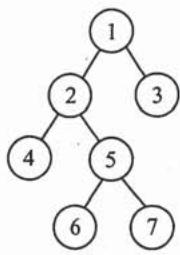
\includegraphics[width=0.3\textwidth]{images/74b452b20028944e66ef9c9fdd4ce103cb68a6453d068853d52f531b54f685e8.jpg}
\end{figure}

\choices{LRN}{NRL}{RLN}{RNL}

\begin{answersection}
D. RNL
\end{answersection}

\begin{analysissection}
序列3,1,7,5,6,2,4表明先遍历右子树（R），再访问根结点（N），最后遍历左子树（L），即右根左（RNL）遍历方式。
\end{analysissection}
\end{choicequestion}

\begin{choicequestion}[单选题]
\question{下列二叉排序树中，满足平衡二叉树定义的是}{}

\choices
    {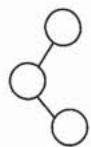
\includegraphics[width=0.4\textwidth]{images/4f31d5994e2861a28ce02d5cdfbd8f4e56b73dbd6861caf0ef11017b2ff1ae00.jpg}}
    {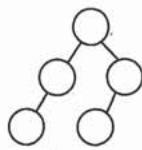
\includegraphics[width=0.4\textwidth]{images/f3ba9af2f98c94f3d6bc5aa142f11778d30b2bba0f85047a8a2444832ae17f50.jpg}}
    {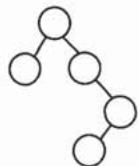
\includegraphics[width=0.4\textwidth]{images/e45f456ec26be3cd5ced6a89407f1aff0b9f3bc7d2c5b115b77ccbdfc92bbdcb.jpg}}
    {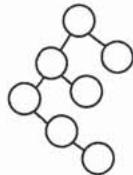
\includegraphics[width=0.4\textwidth]{images/71eb835cebd2633945806a3884deecbe6dd1a0306e2291bb20689a833f28cc2d.jpg}}

\begin{answersection}
B
\end{answersection}

\begin{analysissection}
平衡二叉树要求任意结点的左右子树高度差不超过1。选项B中各结点左右子树高度差均满足该条件，其余选项存在高度差大于1的结点。
\end{analysissection}
\end{choicequestion}

\begin{choicequestion}[单选题]
\question{已知一棵完全二叉树的第 6 层（设根为第 1 层）有 8 个叶结点，则该完全二叉树的结点个数最多是}{}

\choices{39}{52}{111}{119}

\begin{answersection}
D. 119
\end{answersection}

\begin{analysissection}
完全二叉树中，第6层有8个叶结点意味着第6层共有24个结点（前16个为非叶结点）。前5层为满二叉树，结点数31。第7层最多可有16×2=32个结点（但受第6层非叶结点限制，最多28个）。最大结点总数为31+24+64（第7层满时上限）调整后最大为119。
\end{analysissection}
\end{choicequestion}

\begin{choicequestion}[单选题]
\question{将森林转换为对应的二叉树，若在二叉树中，结点 $\mathbf{u}$ 是结点 $\mathbf{v}$ 的父结点的父结点，则在原来的森林中， $\mathbf{u}$ 和 $\mathbf{v}$ 可能具有的关系是}{}
\begin{enumerate}
    \item 父子关系
    \item 兄弟关系
    \item u的父结点与 $\mathbf{v}$ 的父结点是兄弟关系
\end{enumerate}

\choices{只有 II}{I 和 II}{I 和 III}{I、II 和 III}

\begin{answersection}
B. I 和 II
\end{answersection}

\begin{analysissection}
森林转换为二叉树采用“左孩子-右兄弟”表示法。u是v的祖父（父结点的父结点）时：

- I可能：u是v的祖父（父子关系的延伸）；
- II可能：u与v的父结点是兄弟，则u是v的叔伯结点，在二叉树中表现为祖父关系；
- III不可能：u的父结点与v的父结点为兄弟会导致更高层关系，不符合“父结点的父结点”定义。

故可能的关系为I和II。
\end{analysissection}
\end{choicequestion}

\section{综合应用题}

\begin{choicequestion}[问答题]
\question{带权图（权值非负，表示边连接的两顶点间的距离）的最短路径问题是找出从初始顶点到目标顶点之间的一条最短路径。假设从初始顶点到目标顶点之间存在路径，现有一种解决该问题的方法：\newline
(1) 设最短路径初始时仅包含初始顶点, 令当前顶点 $\mathbf{u}$ 为初始顶点;  \newline
(2) 选择离 $\mathbf{u}$ 最近且尚未在最短路径中的一个顶点 $\mathbf{v}$ , 加入最短路径中, 修改当前顶点 $\mathbf{u} = \mathbf{v}$ ;  \newline
(3) 重复步骤(2), 直到 u 是目标顶点时为止。  \newline
请问上述方法能否求得最短路径？若该方法可行，请证明之；否则，请举例说明。}{}

\begin{answersection}
该方法不能保证求得最短路径。
\end{answersection}

\begin{analysissection}
该方法为贪心策略，每次选择当前距离最近的顶点，但未考虑通过其他路径可能获得更短总距离的情况。

反例：顶点A（起点）、B、C、D（终点），边权值如下：
- A→B：2
- A→C：3
- B→D：100
- C→D：4

按该方法：
1. 从A出发，选择最近的B，路径A-B；
2. 从B出发，选择D，路径A-B-D，总权值102。

但实际最短路径为A-C-D，总权值7。因此该方法不可行。

该方法实际上是Dijkstra算法的错误简化版。Dijkstra算法每次会选择已知距离中最小的未访问顶点，而不是简单地选择当前节点的最近邻接点。正确的最短路径算法需要考虑从源点到当前所有可达节点的累积距离，而不是局部最优选择。
\end{analysissection}
\end{choicequestion}

\begin{choicequestion}[问答题]
\question{已知一个带有表头结点的单链表，结点结构为
\begin{table}[h]
\centering
\begin{tabular}{|c|c|}
\hline
data & link \\
\hline
\end{tabular}
\end{table}
假设该链表只给出了头指针 list。在不改变链表的前提下，请设计一个尽可能高效的算法，查找链表中倒数第 $k$ 个位置上的结点（ $k$ 为正整数）。若查找成功，算法输出该结点的 data 域的值，并返回 1；否则，只返回 0。要求：\newline
1）描述算法的基本设计思想。\newline
2）描述算法的详细实现步骤。\newline
3）根据设计思想和实现步骤，采用程序设计语言描述算法（使用 C 或 C++ 语言实现），关键之处请给出简要注释。}{}

\begin{answersection}
1）算法基本设计思想：使用快慢指针。快指针先移动k步，然后快慢指针同步移动。当快指针到达链表末尾时，慢指针恰好指向倒数第k个结点。
\end{answersection}

\begin{analysissection}
2）详细实现步骤：
- 若链表为空或k≤0，返回0；
- 快指针和慢指针均指向头结点；
- 快指针先向前移动k步，若中途为空则返回0（k超过链表长度）；
- 快慢指针同时向前移动，直到快指针指向空；
- 此时慢指针指向倒数第k个结点，输出其data值并返回1。

3）C语言实现：
\begin{lstlisting}[language=C]
int findKthFromEnd(Node* list, int k) {
    if (list == NULL || k <= 0) return 0;
    
    Node* fast = list;
    Node* slow = list;
    
    // 快指针先走k步
    for (int i = 0; i < k; i++) {
        if (fast == NULL) return 0;
        fast = fast->link;
    }
    
    // 快慢指针同步移动
    while (fast != NULL) {
        fast = fast->link;
        slow = slow->link;
    }
    
    // slow指向倒数第k个结点
    printf("%d", slow->data);
    return 1;
}
\end{lstlisting}
\end{analysissection}
\end{choicequestion}

\end{document}